\section{Charged leptons in cosmic plasma - CTY}\label{Electron}

Charged leptons played significant roles in the dynamics and evolution of the early Universe. They were kept in equilibrium via electromagnetic and weak interactions.  In this chapter, I examine a dynamical model of the abundance of charged leptons $\mu^\pm$ and $e^\pm$ in the early Universe obtaining their disappearance temperature, the condition when they disappear from the particle inventory. Of particular interest is the dense electron-positron plasma present during the early Universe evolution. I study the damping rate and the magnetization process in this dense $e^\pm$ plasma in the early Universe.


%{Introduction\daggerfootnote{This chapter has been published previously as \citet{Gottbrath1999}.}}
%~~~~~~~~~~~~~~~~~~~~~~~~~~~~~~~~~~~~~~~~~~~~~~~~~

\section{Overview of charge leptons in early Universe}
%In this section we will focus on the following:
%\begin{itemize}
%    \item Charged leptons in early universe
%    \item Remarks on tau leptons
%\end{itemize}


%In the early universe, charged leptons are kept equilibrium with the cosmic plasma via electromagnetic and weak interactions which played significant roles in the dynamics and evolution of the Universe.  For example, the present $e^\pm$ in early universe can affect  the neutrino decoupling, photon heating, and big bang nucleosynthesis. Although, the massive lepton $\tau^\pm, \mu^\pm$ decay into light leptons ($\nu$, $l^\pm$) and hadrons in their lifespan. These high-energy leptons ($\nu$, $l^\pm$) originating from the decay of $\tau^\pm, \mu^\pm$ continue played a significant role in shaping the particle energy distribution which can affect the property of cosmic plasma.



The $\tau^\pm$ leptons can undergo various decay processes via the weak interaction in the early Universe, and is the only charged lepton that can decay into hadrons because of its heavy mass ($m_\tau=1776.86$ MeV). The principle decay channels of $\tau^\pm$ are given by
\begin{align}
&\tau^-\rightarrow\nu_\tau+e^-+\bar{\nu}_e,\qquad \tau^-\rightarrow\nu_\tau+\mu^-+\bar{\nu}_\mu,\\
&\tau^-\rightarrow\nu_\tau+\pi^-,\qquad\qquad\,\tau^+\rightarrow\bar{\nu}_\tau+\pi^+,
\end{align}
 where the vacuum lifespan for $\tau^\pm$ is given by ~[\cite{ParticleDataGroup:2022pth}]
\begin{align}
&\tau_{\tau}=(290.3\pm0.5)\times10^{-15}\,\mathrm{sec}.
\end{align}

Moreover, following the decay of $\tau^\pm$ into pions, these pions subsequently decay into a muon and a neutrino through the reaction
\begin{align}
\pi^-\rightarrow\nu_\mu+\mu^-,\qquad\qquad\,\pi^+\rightarrow\bar{\nu}_\mu+\mu^+,
\end{align}
with pion vacuum lifespan $\tau_\pi=2.6033\times10^{-8}$ sec~[\cite{ParticleDataGroup:2022pth}].
In this scenario, $\tau^\pm$ disappears from the Universe via multiparticle decay processes.
These decay processes can contribute as one of the sources for the production of neutrinos and muons in the early Universe.

The $\mu^\pm$ lepton abundance is an important quantity required for the understanding of several fundamental questions regarding properties of the primordial Universe,  particularly in relation to the freeze-out of strangeness flavor in the early Universe. We recall that the strangeness decay often proceeds into muons, energy thresholds permitting, as the charged kaons K$^\pm$ have a 63\% branching into $\mu+\bar \nu_\mu$. Should muons fall out of thermal abundance equilibrium this would directly impact the detailed balance back-reaction processes. Another, indirect influence on strangeness in early Universe arises through the nearly exclusive decay of charged pions into $\mu+\bar \nu_\mu$. Without chemical abundance equilibrium this back reaction stops too impacting pions and thus all other hadronic particles in the Universe. 

On the other hand, we will show that the lightest charged leptons $e^\pm$ can persist via the reaction $\gamma\gamma\to e^-e^+$ until the temperature $T=20$ keV in the early Universe.  After $T=20$ keV, the positron rapidly disappears through annihilation, leaving only residual electrons to maintain the Universe's charge neutrality. The existence of an electron-positron plasma plays a pivotal role in several aspects of the early Universe as follows: 

1. The role of electron-positron plasma has not received the appropriate attention in the days of precision Big-Bang nucleosynthesis studies. The standard BBN model indicates that the synthesis of light elements typically takes place at temperatures around  $86\,\mathrm{keV}>T_{BBN}>50\,\mathrm{keV}$~[\cite{Pitrou:2018cgg}]. Within this temperature range there are millions of electron-positron pairs per charged nucleon, providing an electron-positron-rich plasma environment for nucleosynthesis which leads to modifications in the Coulomb potential due to the screening effect. Furthermore, the electron-positron densities can reach millions of times normal atomic densities. The presence of  these $e\bar e$-pairs before and during BBN has been acknowledged by Wang, Bertulani and Balantekin~[\cite{Wang:2010px}] nearly a decade ago.

2. The Universe today is filled with magnetic fields at various scales and strengths both within galaxies and in deep extra-galactic space. The origin of these magnetic fields is currently unknown. In the early Universe, when temperature $T>20$ keV, we have dense $e^\pm$ plasma. The significant magnetic moments of electrons and positrons also provide opportunities to investigate spin magnetization process.

Understanding the abundances of muons and electrons/positrons provides essential insights into the evolution of the primordial Universe.  In the following we discuss the muon density at persistence temperature in section \ref{section_muon}, and explore the electron/positron plasma properties, including the damped rate and magnetization in section \ref{section_electron}.

%~~~~~~~~~~~~~~~~~~~~~~~~~~~~~~~~~~~~~~~~~~~~~~~~~

\section{Muon–antimuon in the early Universe}\label{section_muon}
%In this section we will focus on the following:
%\begin{itemize}
%    \item Vanishing of muon in early Universe
%    \item Muon density at persistence temperature
%\end{itemize}

%\subsection{Vanishing of muon in early Universe}
Our interest in strangeness flavor freeze-out in the early Universe requires the understanding of the abundance of muons in the early Universe. The specific question needing an answer is at which temperature muons remain in abundance (chemical) equilibrium established predominantly by electromagnetic and weak interaction processes, allowing detailed-balance back-reactions to influence strangeness abundance.


In the early Universe in the the cosmic plasma muons of mass $m_\mu=105.66$\,MeV can be produced by the following interaction processes
\begin{align} 
&\gamma+\gamma\longrightarrow\mu^++\mu^-,\qquad & e^++e^-\longrightarrow \mu^++\mu^-\;,\\
&\pi^-\longrightarrow\mu^-+\bar{\nu}_\mu,\qquad & \pi^+\longrightarrow\mu^++\nu_\mu\;.
\end{align}
The back reactions for all above processes are in detailed balance, provided all particles shown on the right hand side (RHS) exist in chemical abundance equilibrium in the Universe. We recall the empty space (no plasma) at rest lifetime of pions $\tau_\pi=2.6033\times10^{-8}$ sec. 

However, all produced muons can also decay via the reactions
\begin{equation}
\mu^-\rightarrow\nu_\mu+e^-+\bar{\nu}_e,\qquad \mu^+\rightarrow\bar{\nu}_\mu+e^++\nu_e\,,
\end{equation} 
with the empty space (no plasma) at rest lifetime $\tau_{\mu}=2.197 \times 10^{-6}\,\mathrm{sec}$. We thus must establish the range of temperature in which production processes exceed in speed the decay process.
 
 The temperature range of our interests is the Universe when $m_\mu\gg T$. In this case the the Boltzmann approximation is appropriate for studying massive particles muons and pions. The thermal decay rate per volume and time  for muons $\mu^\pm$ (and pions $\pi^\pm$) in the Boltzmann limit  are given by~[\cite{PhysRevC.82.035203}]:
\begin{align}
&R_\mu=\frac{g_\mu}{2\pi^2}\left(\frac{T^3}{\tau_\mu}\right)\left(\frac{m_\mu}{T}\right)^2K_1(m_\mu/T)\;,\\
&R_\pi=\frac{g_\pi}{2\pi^2}\left(\frac{T^3}{\tau_\pi}\right)\left(\frac{m_\pi}{T}\right)^2K_1(m_\pi/T)\;, 
\end{align}
where the lifespan of $\mu^\pm$ and $\pi^\pm$ in the vacuum were given above. This rate accounts for both the density of particles in chemical abundance equilibrium and the effect of time dilation present when particles are in thermal motion with respect to observer at rest in the local reference frame. The effects of Fermi blocking or boson stimulated emission have been neglected.

The thermal averaged reaction rate per volume for the reaction $a\overline{a}\rightarrow b\overline{b}$ in Boltzmann approximation is given by [\cite{Letessier:2002ony}]
\begin{align}\label{pairR}
R_{a\overline{a}\rightarrow b\overline{b}}=\frac{g_ag_{\overline{a}}}{1+I}\frac{T}{32\pi^4}\int_{s_{th}}^\infty ds\frac{s(s-4m^2_a)}{\sqrt{s}}\sigma_{a\overline{a}\rightarrow b\overline{b}}~K_1(\sqrt{s}/T),
\end{align}
where $s_{th}$ is the threshold energy for the reaction, $\sigma_{a\overline{a}\rightarrow b\overline{b}}$ is the cross section for the given reaction, and $K_1$ is the modified
Bessel function of integer order ``$1$". We introduce the factor $1/1+I$ to avoid the double counting of indistinguishable pairs of particles; we have $I=1$ for an identical pair and $I=0$ for a distinguishable pair.

The leading order invariant matrix elements for the reactions $e^++e^-\to\mu^++\mu^-$ and $\gamma+\gamma\to\mu^++\mu^-$, are introduced in this work by [\cite{Kuznetsova:2008jt}]
\begin{align}\label{Mee}
|M_{e\bar e\to\mu\bar\mu}|^2=&32\pi^2\alpha^2\frac{(m_\mu^2-t)^2+(m_\mu^2-u)^2+2m_\mu^2s}{s^2},\quad m_\mu\gg m_e\;,\\[0.2cm]
\label{Mgg}
|M_{\gamma\gamma\to\mu\bar\mu}|^2=&32\pi^2\alpha^2\bigg[\left(\frac{m_\mu^2-u}{m_\mu^2-t}+\frac{m_\mu^2-t}{m_\mu^2-u}\right)+4\left(\frac{m_\mu^2}{m_\mu^2-t}+\frac{m_\mu^2}{m^2_\mu-u}\right)\\[0.1cm]  \nonumber
&\hspace{1cm}-4\left(\frac{m_\mu^2}{m^2_\mu-t}+\frac{m^2_\mu}{m^2_\mu-u}\right)^2\bigg]\;,
\end{align}
 where $s, t, u$ are the Mandelstam variables. The cross section required in Eq.\,(\ref{pairR}) can be obtained by integrating the matrix elements Eq.\,(\ref{Mee}) and Eq.\,(\ref{Mgg}) over the Mandelstam variable $t$ ~[\cite{PhysRevC.82.035203}]. We have
\begin{align}
&\sigma_{e\bar e\to\mu\bar\mu} 
=\frac{64\pi\alpha^2}{48\pi}\left(\frac{1+2m^2_\mu/s}{s-4m_e^2}\right)\sqrt{1-\frac{4m^2_\mu}{s}},\\
&\sigma_{\gamma\gamma\to\mu\bar\mu}=\frac{\pi}{2}\left(\frac{\alpha}{m_\mu}\right)^2(1-\beta^2)\left[(3-\beta^4)\ln\frac{1+\beta}{1-\beta}-2\beta(2-\beta^2)\right],\\
&\beta=\sqrt{1-4m^2_\mu/s}
\end{align}
Substituting the cross sections into Eq.\,(\ref{pairR}) we obtain the production rates for $e\bar e\to\mu\bar\mu$ and $\gamma\gamma\to\mu\bar\mu$ respectively.

 
In Fig.~\ref{MuonRatenew_fig} we show the invariant thermal reaction rates per volume and time for rates of relevance, as a function of temperature $T$.
As the temperature decreases in the expanding Universe, the initially dominant production rates ($e\bar e,\gamma\gamma\to\mu\bar\mu$) decrease with decreasing temperature, and eventually cross the $\mu^\pm$ decay rates. 
Muon abundance disappears as soon as any decay rate is faster than the fastest production rate. Specifically after the Universe cools below the temperature $T_\mathrm{disappear}=4.195$ MeV, the dominant reaction is the muon decay. Due to the relatively slow expansion of the Universe, the disappearance of muons is sudden, and the abundance of muons vanishes as soon as a decay rate surpasses the dominant production rate.
 

%~~~~~~~Figure~~~~~~ ~~~~~~~~~~~~~~~~~~~~~~~~~~~~~~~~~~~~~~~~~~~~~~~~~~~~~~~~~~~~~~~~~~~
\begin{figure}[ht]
\begin{center}
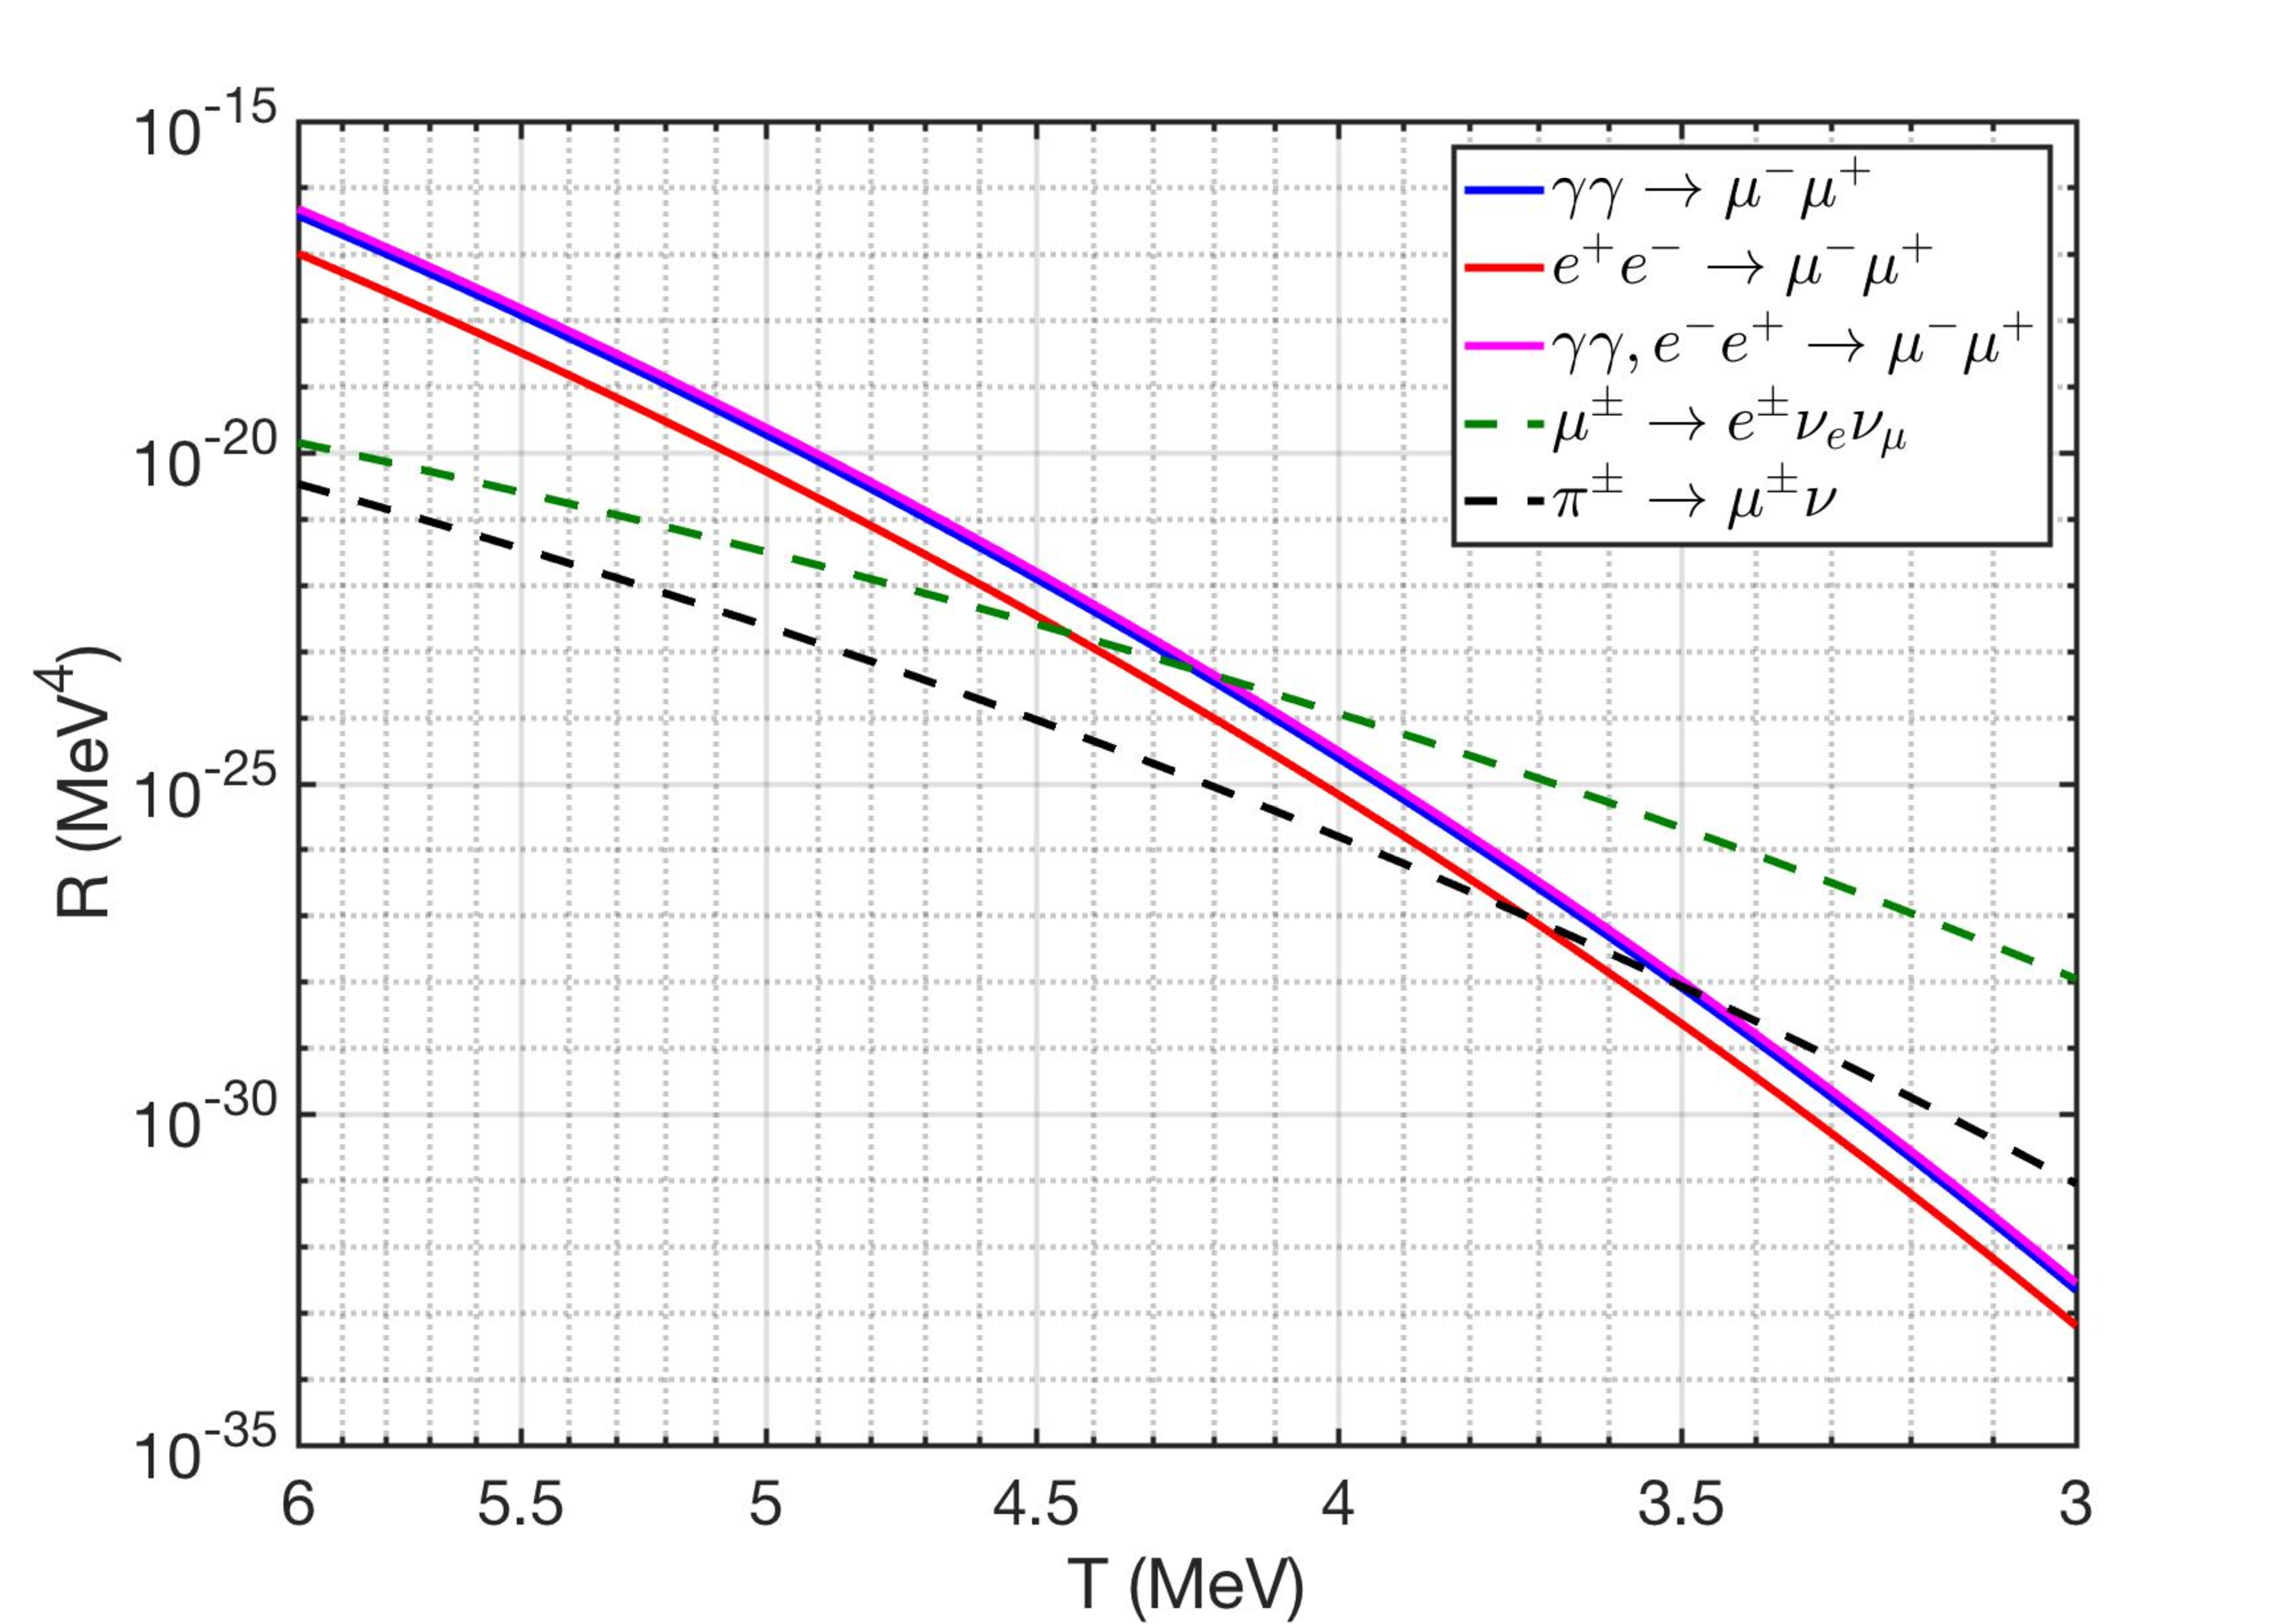
\includegraphics[width=5.0in]{./plots/MuonRate_new2.pdf}
\caption{We plot the thermal reaction rate per volume for different reactions as a function of temperature. We found that dominant reactions for $\mu^\pm$ production are ${\gamma+\gamma\to\mu^++\mu^-}$ and $e^++e^-\to\mu^++\mu^-$, and the total production rate crosses the decay rate of $\mu^\pm$ at temperature $T_{dissapear}\approx 4.195$ MeV.}
\label{MuonRatenew_fig}
\end{center}
\end{figure}
%~~~~~~~~~~~~~~~~~~~~~~~~~~~~~~~~~~~~~~~~~~~~~~~~~~~~~~~~~~~~~~~~~~~~~~~~~~~~~~~~~~~~~~~~~~~~~~~~

On the other hand, considering the number density for nonrelativistic $\mu^\pm$ in the Boltzmann approximation, we have
\begin{align}\label{nmupm}
n_{\mu^\pm}=\frac{g_{\mu^\pm}}{2\pi^2}T^3\left(\frac{m_\mu}{T}\right)^2 K_2(m_\mu/T)=g_{\mu^\pm}\left(\frac{m_\mu T}{2\pi}\right)^{3/2}e^{-{m_\mu}/{T}}\;. 
\end{align}
then the number density between $n_{\mu^\pm}$ and baryon $n_B$ can be written as
\begin{align}
\frac{n_{\mu^\pm}}{n_\mathrm{B}}=\frac{n_{\mu^\pm}}{s}\frac{s}{n_\mathrm{B}}=
\frac{n_{\mu^\pm}}{s}\left(\frac{s}{n_\mathrm{B}}\right)_{\!t_0},
\end{align}
where we used that $s/n_\mathrm{B}$ remains constant and $t_0$ represent present day value. The present value is given by $(n_B/s)_{t_0}\approx8.69\times10^{-11}$ (detail please see Chapter~\ref{Introduction}). The entropy density $s$ can be characterized introducing $g^s_\ast$, the total number of \lq entropic\rq\ degrees of freedom
\begin{align}\label{entrop}
s=\frac{2\pi^2}{45}g^s_\ast T^3\;.
\end{align}
For temperature $10\,\mathrm{MeV} >T>3 $\,MeV, the massless photons, nearly relativistic electron/positrons, and practically massless neutrinos contribute to the degree of freedom $g^s_\ast$.  In this case, the number density between $n_{\mu^\pm}$ and baryon $n_B$ in the temperature interval we consider $10\,\mathrm{MeV} >T>3 $\,MeV is given by
\begin{align}\label{nmuperbF} 
\frac{n_{\mu^\pm}}{n_\mathrm{B}}=\frac{45}{2\pi^2}\frac{g_{\mu^\pm}}{g^s_\ast}\left(\frac{m_\mu}{2\pi T}\right)^{3/2}e^{-{m_\mu}/{T}}\;\left(\frac{s}{n_\mathrm{B}}\right)_{\!t_0}.
\end{align}


%Figure~~~~~~~~~~~~~~~~~~~~~~~~~~~~~~~~~~~~~~~~~~~~~~~~~~~~~~~~~~~~~~~~~~~~~~~~~
\begin{figure}[t]
\begin{center}
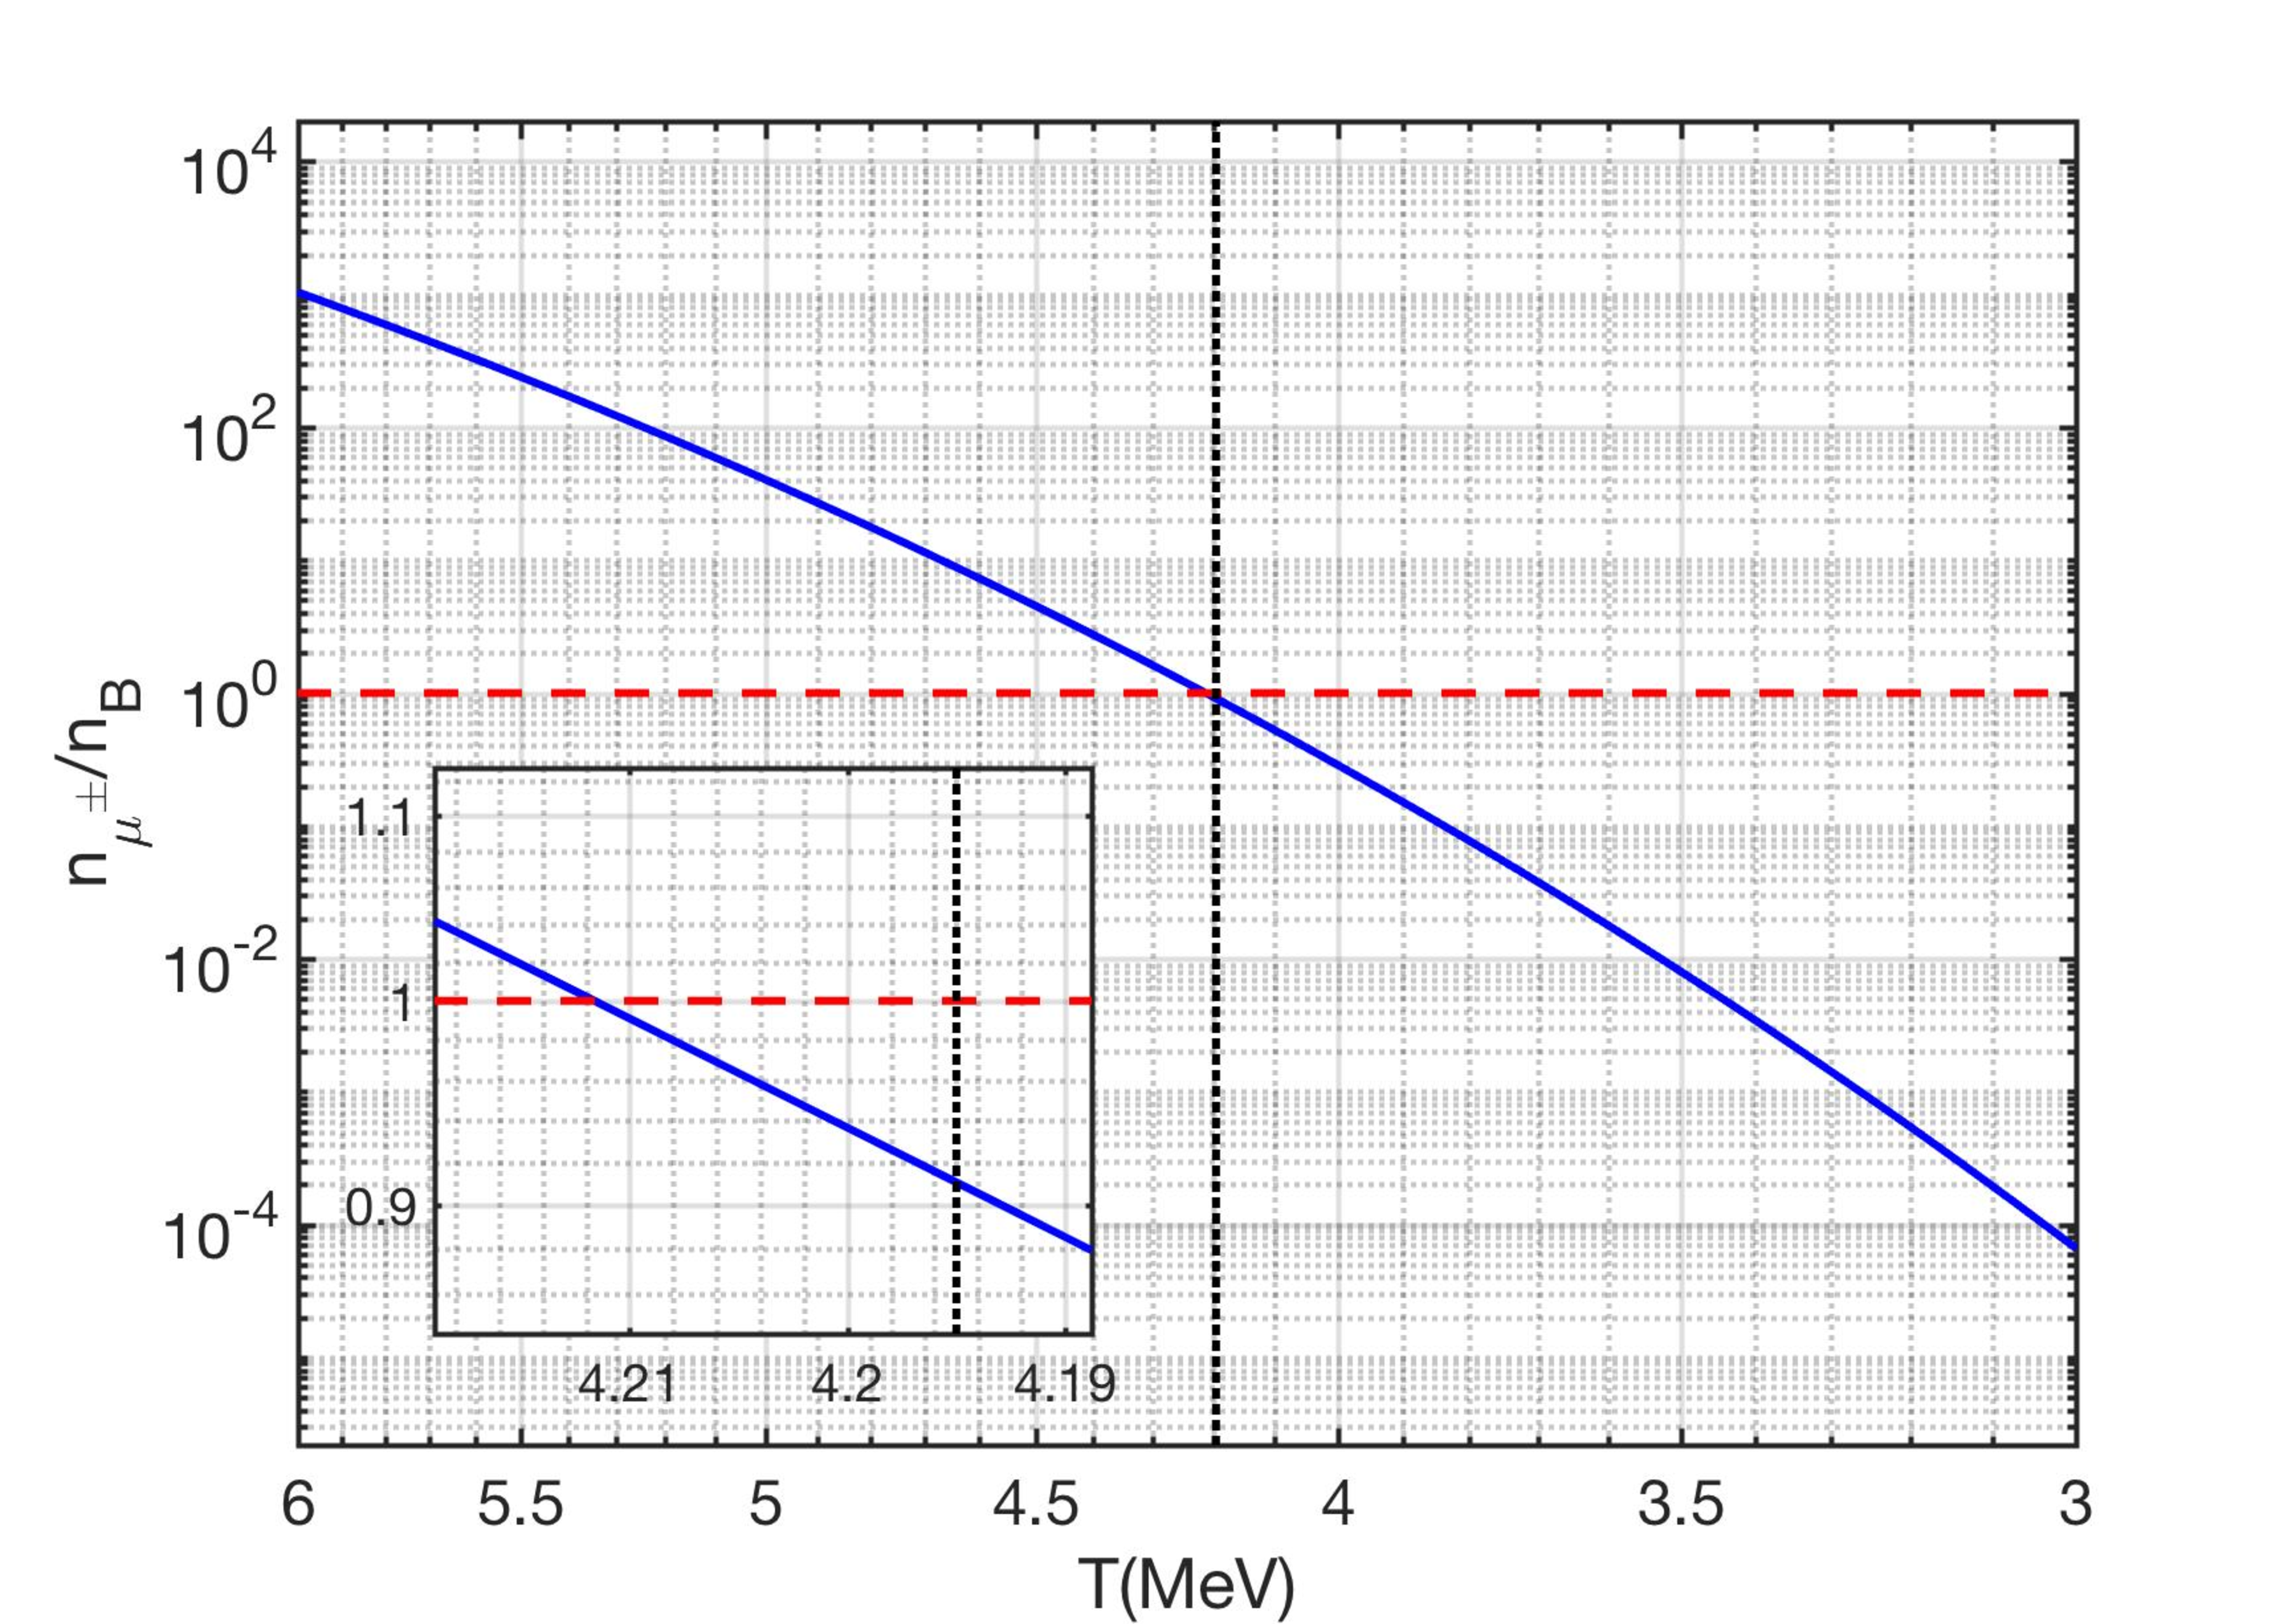
\includegraphics[width=\linewidth]{./plots/DensityRatio_new2.pdf}
\caption{
The density ratio between $\mu^\pm$ and baryons as a function of temperature. The density ratio at muon disappearance temperature is about $n_{\mu^\pm}/n_\mathrm{B}(T_\mathrm{disappear})\approx0.911$, and around the temperature $T\approx4.212$ MeV the density ratio $n_{\mu^\pm}/n_\mathrm{B}\approx1$.}
\label{DensityRatio_fig}
\end{center}
\end{figure}
%~~~~~~~~~~~~~~~~~~~~~~~~~~~~~~~~~~~~~~~~~~~~~~~~~~~~~~~~~~~~~~~~~~~~~~~~~~~~~


In Fig.\,\ref{DensityRatio_fig} we show the muon to baryon density ratio Eq.\,(\ref{nmuperbF}) as a function of $T$. We see that the muon abundance $T=10$\,MeV exceeds that of baryons by a factor 500,000 while at muon disappearance temperature $n_{\mu^\pm}/n_\mathrm{B}(T_\mathrm{disappear})\approx0.911$. The number density $n_{\mu^\pm}$ and $n_\mathrm{B}$  abundances are equal at around the temperature $T_\mathrm{equal}\approx4.212\,\mathrm{MeV} >  T_\mathrm{disappear}$.  This means that the muon abundance may still be able to influence baryon evolution because their number density is comparable to the baryon density.% However, we also find that at the temperature $T_\mathrm{equal}\approx4.212$\,MeV the density ratio is unity $n_{\mu^\pm}/n_\mathrm{B}\approx1$.

The primary insight of this work is that aside of protons, neutrons and other nonrelativistic particles, both positively and negatively charged muons $\mu^\pm$ are present in thermal equilibrium and in non-negligible abundance for $T>T_\mathrm{dissapear}\approx 4.195$\,MeV. This offers a new and tantalizing model building opportunity for anyone interested in baryon-antibaryon separation in the primordial Universe, strangelet formation, and perhaps other exotic primordial structure formation mechanisms.
